% Options for packages loaded elsewhere
\PassOptionsToPackage{unicode}{hyperref}
\PassOptionsToPackage{hyphens}{url}
%
\documentclass[
]{article}
\usepackage{amsmath,amssymb}
\usepackage{iftex}
\ifPDFTeX
  \usepackage[T1]{fontenc}
  \usepackage[utf8]{inputenc}
  \usepackage{textcomp} % provide euro and other symbols
\else % if luatex or xetex
  \usepackage{unicode-math} % this also loads fontspec
  \defaultfontfeatures{Scale=MatchLowercase}
  \defaultfontfeatures[\rmfamily]{Ligatures=TeX,Scale=1}
\fi
\usepackage{lmodern}
\ifPDFTeX\else
  % xetex/luatex font selection
\fi
% Use upquote if available, for straight quotes in verbatim environments
\IfFileExists{upquote.sty}{\usepackage{upquote}}{}
\IfFileExists{microtype.sty}{% use microtype if available
  \usepackage[]{microtype}
  \UseMicrotypeSet[protrusion]{basicmath} % disable protrusion for tt fonts
}{}
\makeatletter
\@ifundefined{KOMAClassName}{% if non-KOMA class
  \IfFileExists{parskip.sty}{%
    \usepackage{parskip}
  }{% else
    \setlength{\parindent}{0pt}
    \setlength{\parskip}{6pt plus 2pt minus 1pt}}
}{% if KOMA class
  \KOMAoptions{parskip=half}}
\makeatother
\usepackage{xcolor}
\usepackage[margin=1in]{geometry}
\usepackage{graphicx}
\makeatletter
\def\maxwidth{\ifdim\Gin@nat@width>\linewidth\linewidth\else\Gin@nat@width\fi}
\def\maxheight{\ifdim\Gin@nat@height>\textheight\textheight\else\Gin@nat@height\fi}
\makeatother
% Scale images if necessary, so that they will not overflow the page
% margins by default, and it is still possible to overwrite the defaults
% using explicit options in \includegraphics[width, height, ...]{}
\setkeys{Gin}{width=\maxwidth,height=\maxheight,keepaspectratio}
% Set default figure placement to htbp
\makeatletter
\def\fps@figure{htbp}
\makeatother
\setlength{\emergencystretch}{3em} % prevent overfull lines
\providecommand{\tightlist}{%
  \setlength{\itemsep}{0pt}\setlength{\parskip}{0pt}}
\setcounter{secnumdepth}{-\maxdimen} % remove section numbering
\usepackage{booktabs}
\usepackage{longtable}
\usepackage{array}
\usepackage{multirow}
\usepackage{wrapfig}
\usepackage{float}
\usepackage{colortbl}
\usepackage{pdflscape}
\usepackage{tabu}
\usepackage{threeparttable}
\usepackage{threeparttablex}
\usepackage[normalem]{ulem}
\usepackage{makecell}
\usepackage{xcolor}
\ifLuaTeX
  \usepackage{selnolig}  % disable illegal ligatures
\fi
\IfFileExists{bookmark.sty}{\usepackage{bookmark}}{\usepackage{hyperref}}
\IfFileExists{xurl.sty}{\usepackage{xurl}}{} % add URL line breaks if available
\urlstyle{same}
\hypersetup{
  pdftitle={Progress Report},
  pdfauthor={Ying Jin},
  hidelinks,
  pdfcreator={LaTeX via pandoc}}

\title{Progress Report}
\author{Ying Jin}
\date{2023-05-12}

\begin{document}
\maketitle

{
\setcounter{tocdepth}{3}
\tableofcontents
}
\hypertarget{visualization-of-weigts-in-incident-sensitivity}{%
\section{Visualization of weigts in Incident
sensitivity}\label{visualization-of-weigts-in-incident-sensitivity}}

\hypertarget{model-overfit}{%
\subsection{Model overfit}\label{model-overfit}}

\begin{verbatim}
## # A tibble: 30 x 6
## # Groups:   sample, model [6]
##    tid   weight  time model    tbin      sample   
##    <chr>  <dbl> <dbl> <fct>    <fct>     <chr>    
##  1 X51    0.229 0.665 No noise (0.6,0.7] In-sample
##  2 X43    0.221 0.665 No noise (0.6,0.7] In-sample
##  3 X141   0.209 0.664 No noise (0.6,0.7] In-sample
##  4 X40    0.200 0.655 No noise (0.6,0.7] In-sample
##  5 X19    0.197 0.646 No noise (0.6,0.7] In-sample
##  6 X117   0.225 0.977 20 noise (0.9,1]   In-sample
##  7 X51    0.215 0.665 20 noise (0.6,0.7] In-sample
##  8 X43    0.209 0.665 20 noise (0.6,0.7] In-sample
##  9 X141   0.201 0.664 20 noise (0.6,0.7] In-sample
## 10 X136   0.197 0.963 20 noise (0.9,1]   In-sample
## # i 20 more rows
\end{verbatim}

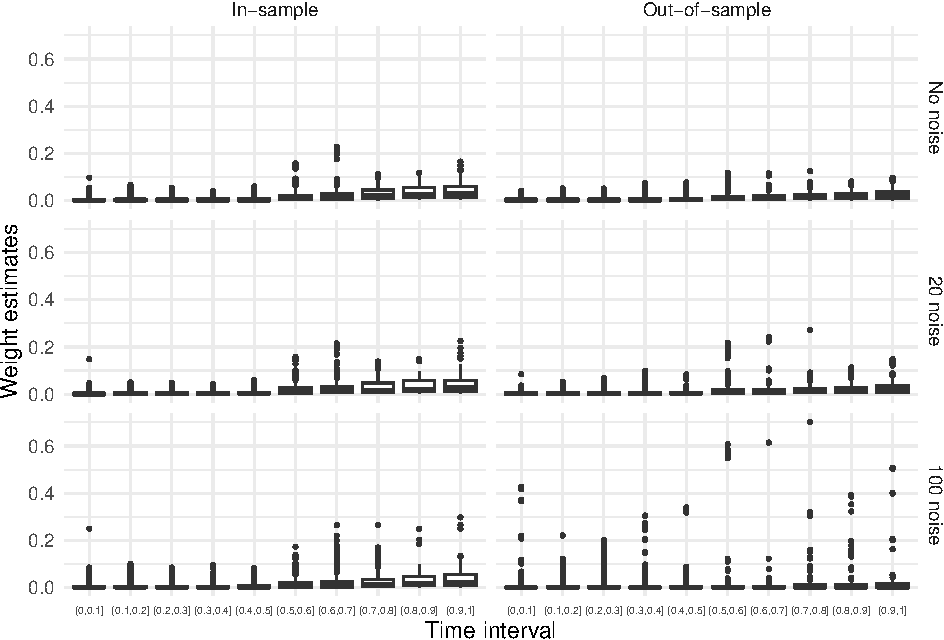
\includegraphics{ProgressReport_files/figure-latex/boxp_wt_noise-1.pdf}

\hypertarget{data-contamination}{%
\subsection{Data contamination}\label{data-contamination}}

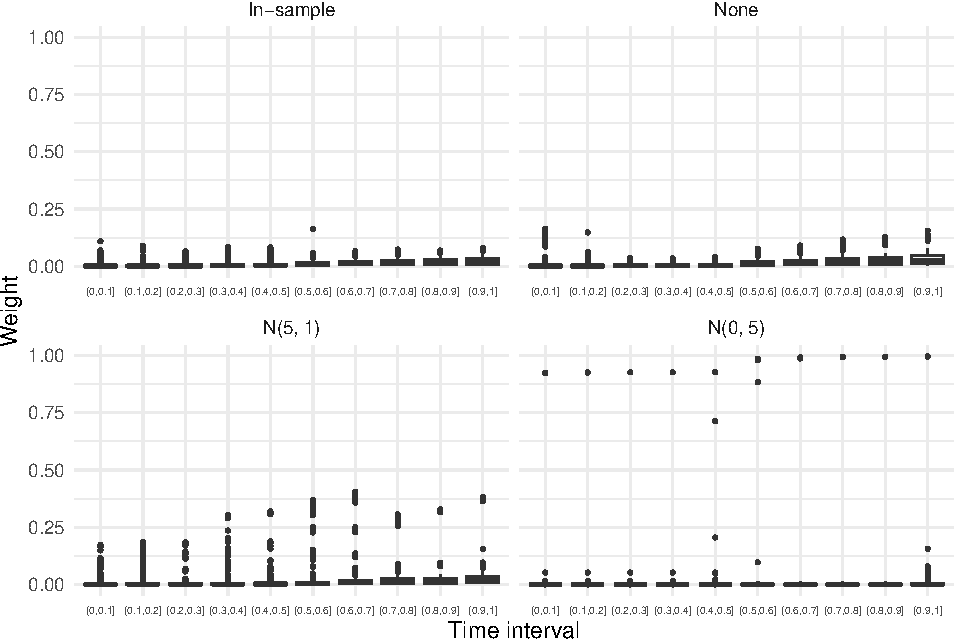
\includegraphics{ProgressReport_files/figure-latex/boxp_wt_contam-1.pdf}

\hypertarget{simulation-with-contaminated-data}{%
\section{Simulation with contaminated
data}\label{simulation-with-contaminated-data}}

\begin{itemize}
\tightlist
\item
  Introduce outliers to test datasets (not noise in the model)
\item
  Modified from last time: instead of arbitrarily change covariate
  value, generate from different random distributions instead
\item
  Within each simulation, two scenarios:
\end{itemize}

\begin{enumerate}
\def\labelenumi{\arabic{enumi}.}
\tightlist
\item
  10\% contaminated subjects, N(5, 1)
\item
  10\% contaminated subjects, N(0, 5)
\end{enumerate}

\begin{itemize}
\tightlist
\item
  Some unexpected coding issue: couldn't find old.alpha parameter in
  scam function (bfgs\_gcv.ubre). Needed to reduce k (k=10).
\end{itemize}

\hypertarget{tv-auc}{%
\subsection{TV-AUC}\label{tv-auc}}

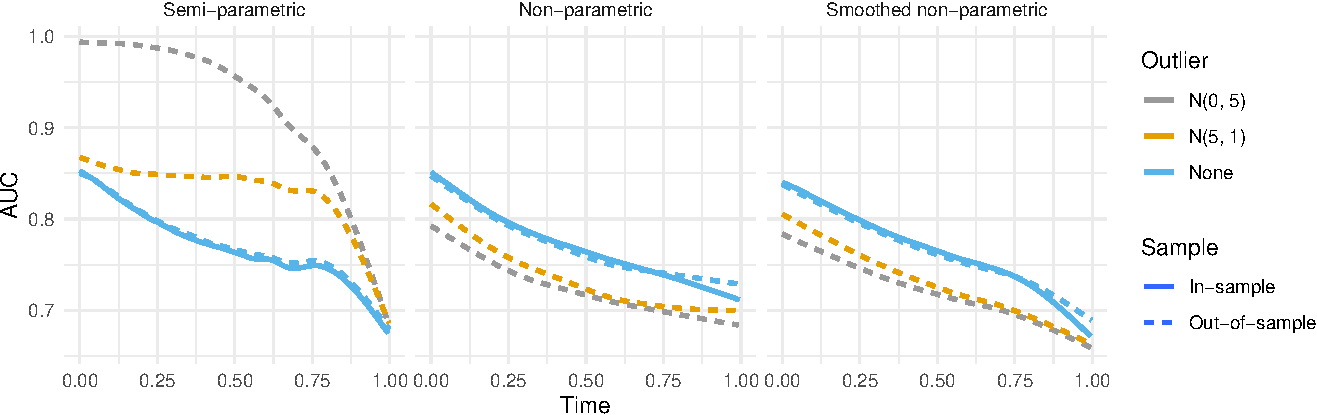
\includegraphics{ProgressReport_files/figure-latex/fig_tv_auc_contam-1.pdf}

\hypertarget{spread-of-tv-auc}{%
\subsection{Spread of TV-AUC}\label{spread-of-tv-auc}}

Do we have alternative ways to present the instability of TV-AUC
estimates? Perhaps remove the figures but only use specific examples:

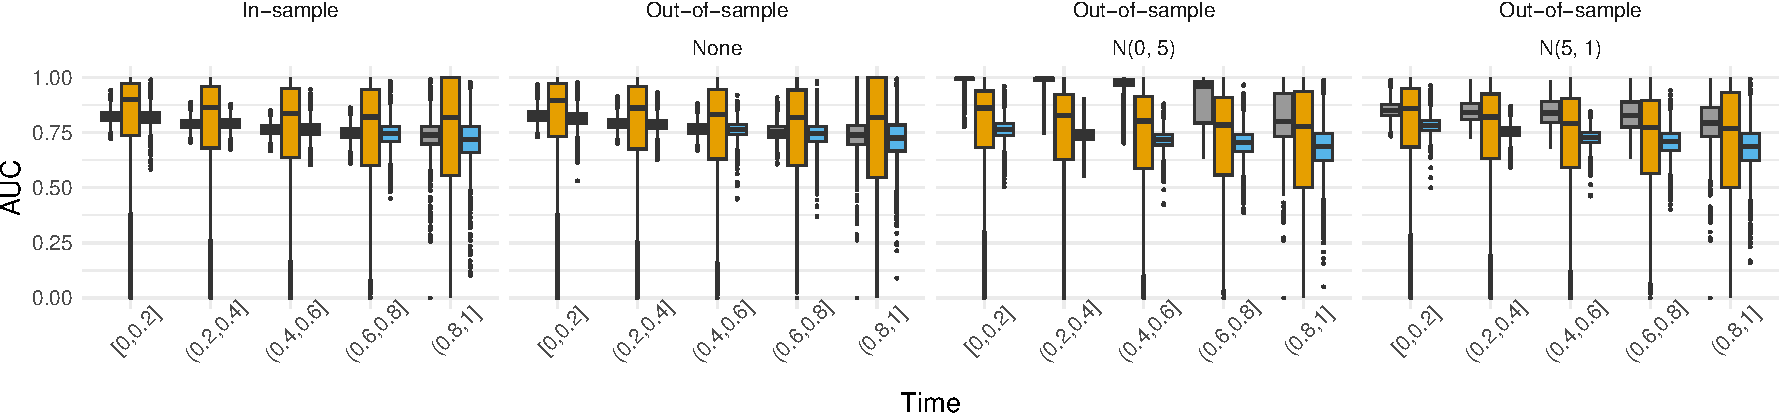
\includegraphics{ProgressReport_files/figure-latex/fig_tvauc_box_contam-1.pdf}

\hypertarget{concordance}{%
\subsection{Concordance}\label{concordance}}

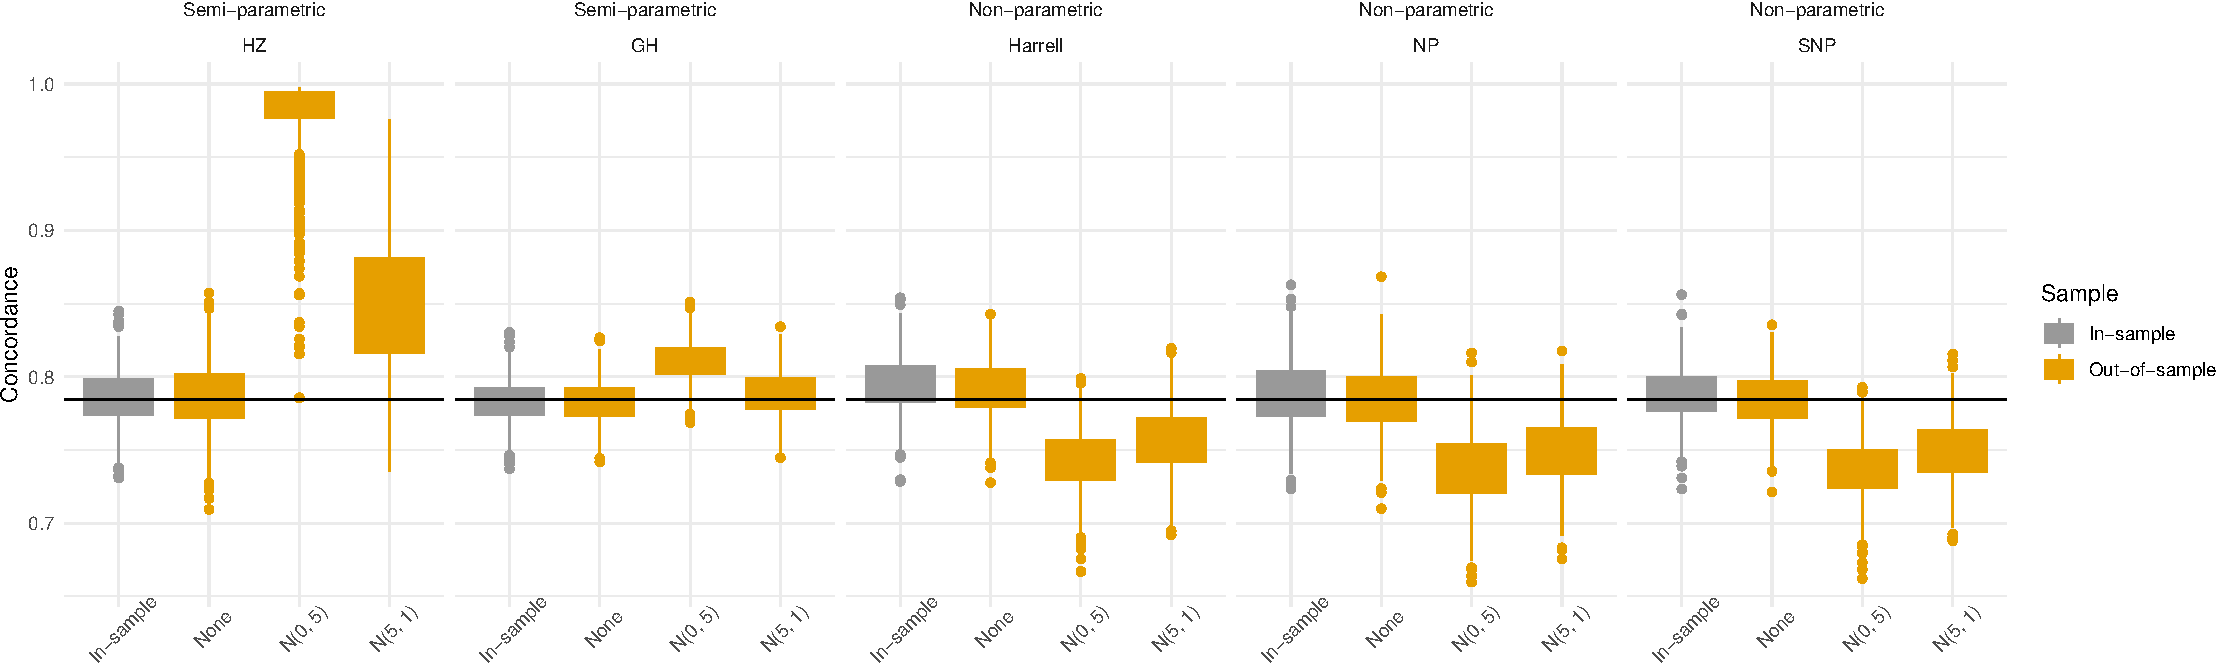
\includegraphics{ProgressReport_files/figure-latex/fig_c_contam-1.pdf}

\hypertarget{simulation-with-noise-signals}{%
\section{Simulation with noise
signals}\label{simulation-with-noise-signals}}

\hypertarget{tv-auc-1}{%
\subsection{TV-AUC}\label{tv-auc-1}}

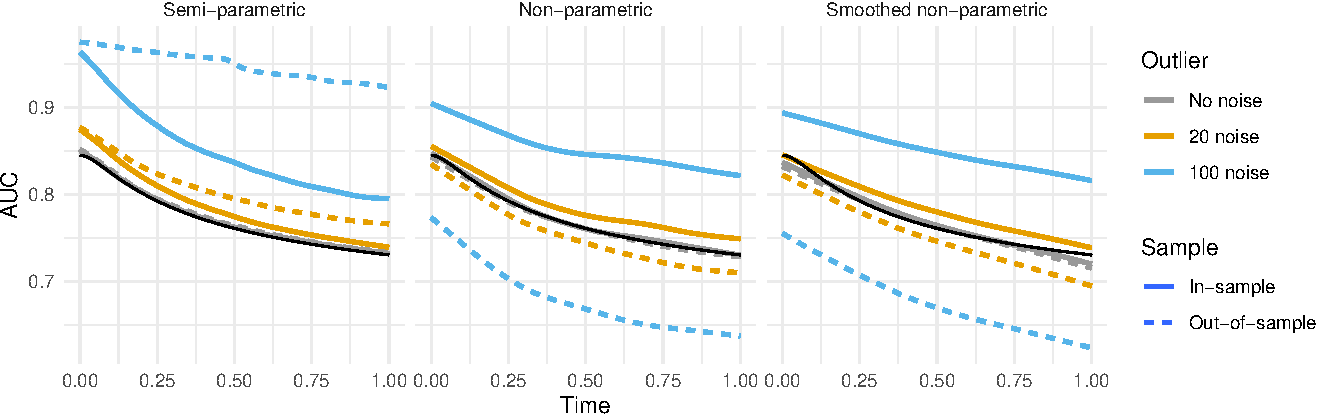
\includegraphics{ProgressReport_files/figure-latex/fig_tv_auc_noise-1.pdf}

\hypertarget{spread-of-tv-auc-1}{%
\subsection{Spread of TV-AUC}\label{spread-of-tv-auc-1}}

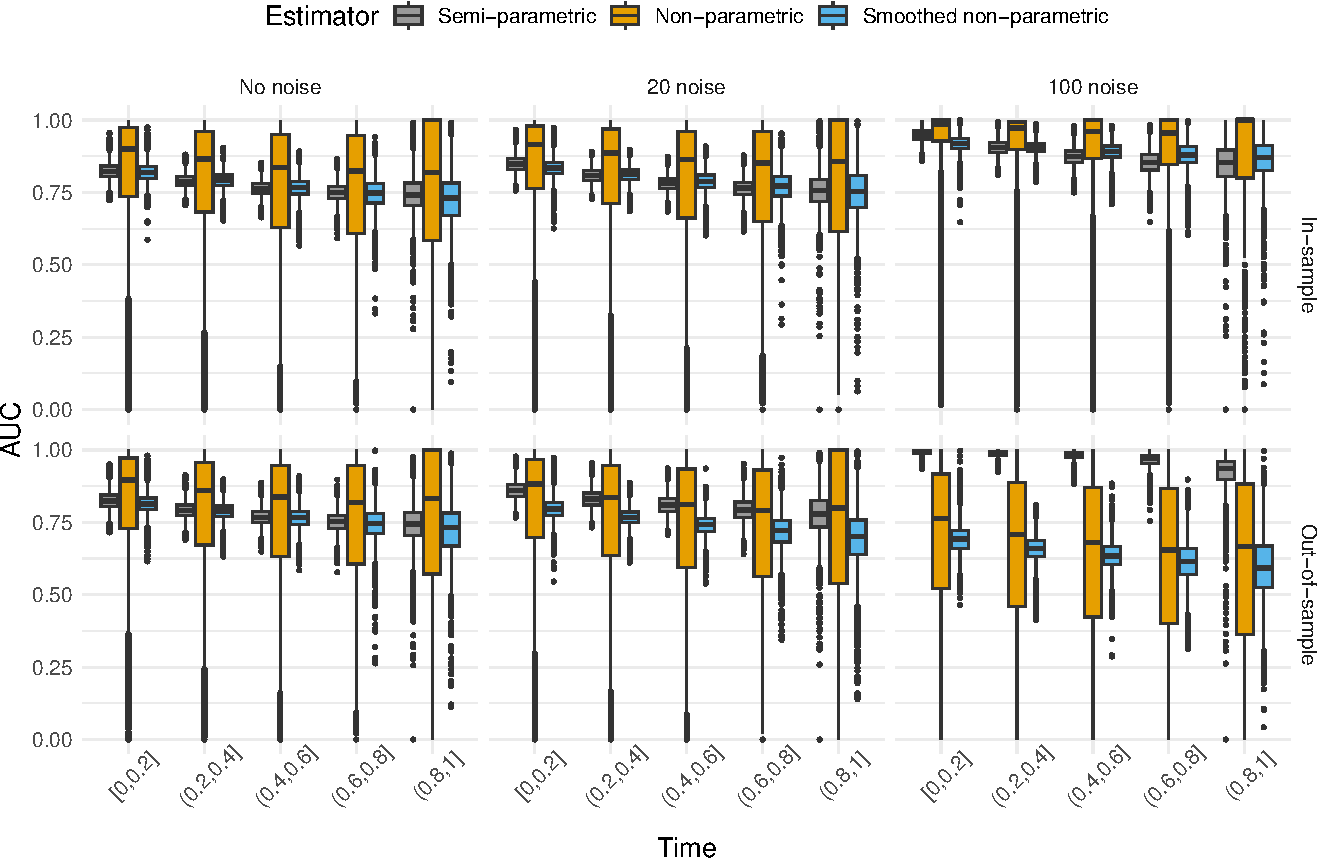
\includegraphics{ProgressReport_files/figure-latex/fig_tvauc_box_ovefit-1.pdf}

\hypertarget{concordance-1}{%
\subsection{Concordance}\label{concordance-1}}

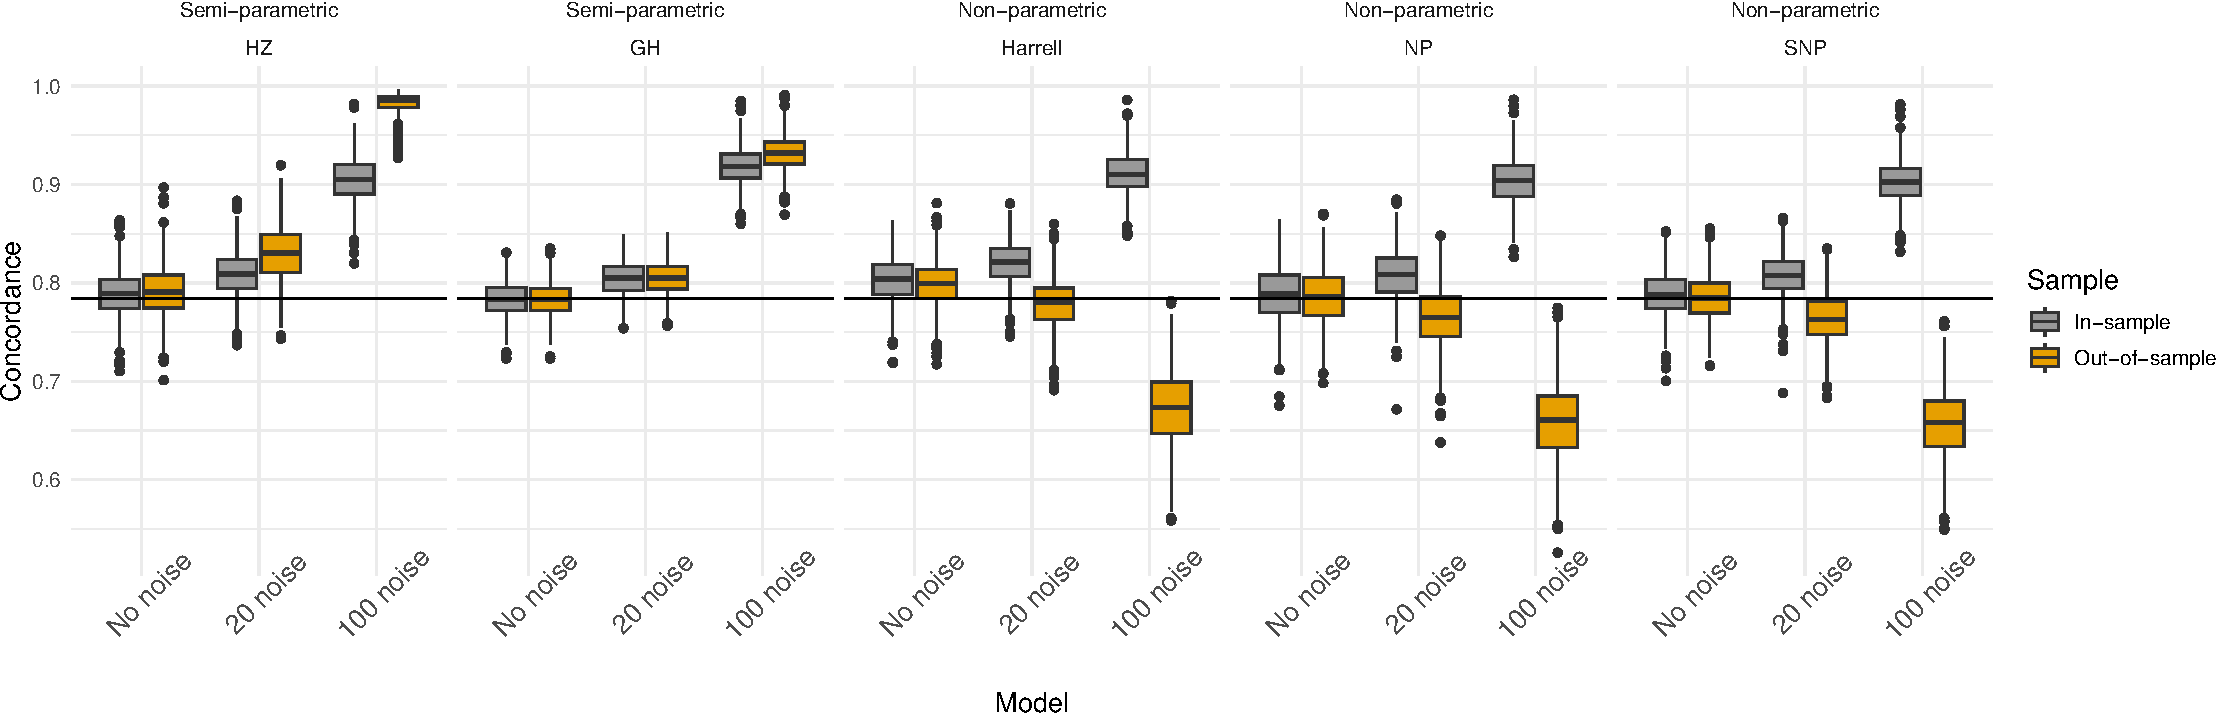
\includegraphics{ProgressReport_files/figure-latex/fig_c_noise-1.pdf}

\hypertarget{data-application}{%
\section{Data Application}\label{data-application}}

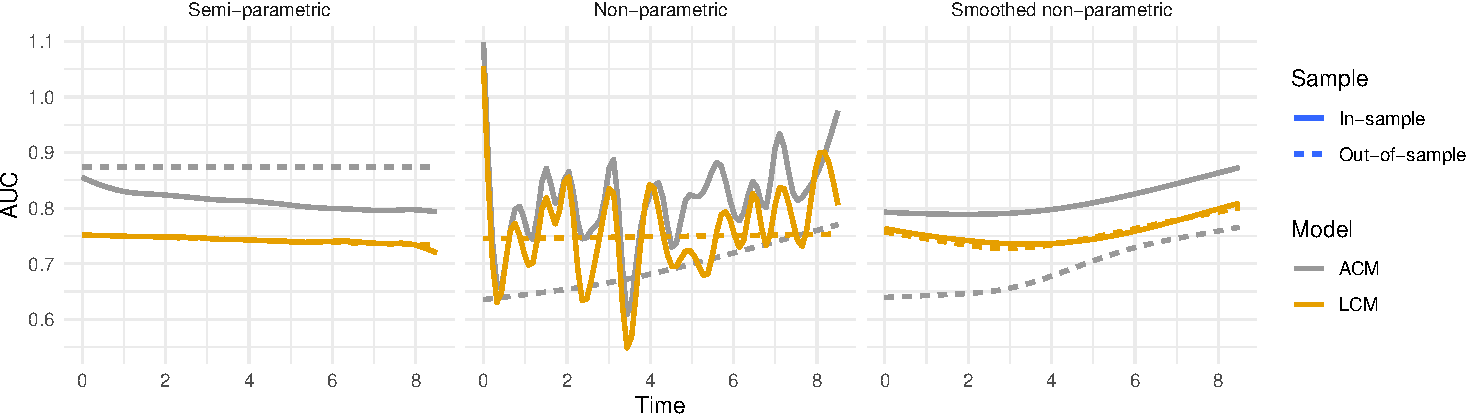
\includegraphics{ProgressReport_files/figure-latex/appl_auc-1.pdf}

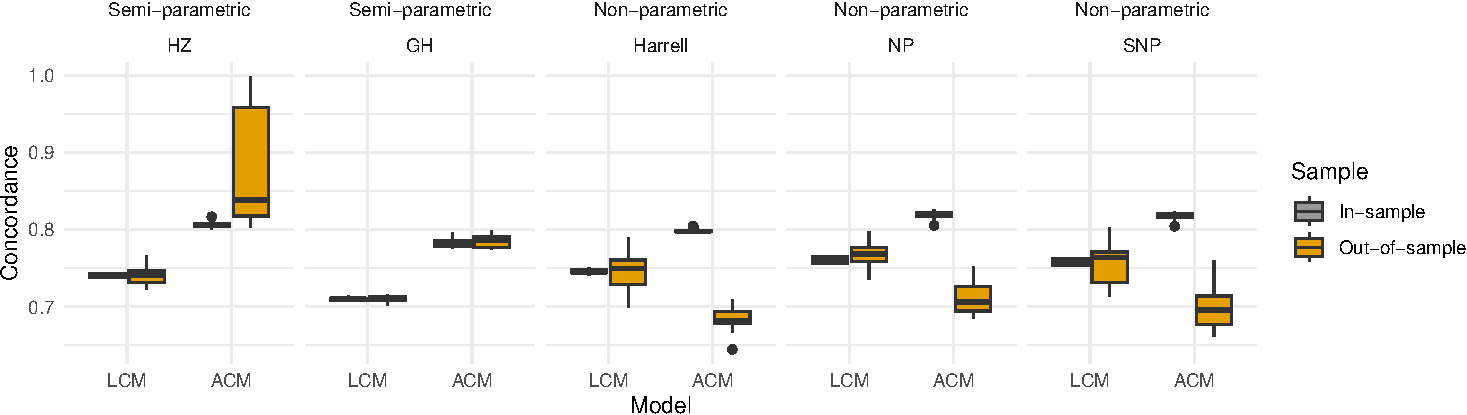
\includegraphics{ProgressReport_files/figure-latex/appl_c-1.pdf}

\hypertarget{summary-table}{%
\section{Summary table}\label{summary-table}}

\begin{verbatim}
## Warning in !is.null(rmarkdown::metadata$output) && rmarkdown::metadata$output
## %in% : 'length(x) = 2 > 1' in coercion to 'logical(1)'
\end{verbatim}

\begin{verbatim}
## 
## Attaching package: 'kableExtra'
\end{verbatim}

\begin{verbatim}
## The following object is masked from 'package:dplyr':
## 
##     group_rows
\end{verbatim}

\begin{table}
\centering
\begin{tabular}{llll}
\toprule
Estimator & Bias & Variavility & Out-of-sample behavior\\
\midrule
\addlinespace[0.3em]
\multicolumn{4}{l}{\textbf{Time-dependent AUC}}\\
\hspace{1em}Semi-parametric & Unbiased & Low & Over-optimistic\\
\hspace{1em}Non-parametric & Unbiased & High & \vphantom{1} Appropriate\\
\hspace{1em}Smoothed non-parametric & Slightly biased & Low & Appropriate\\
\addlinespace[0.3em]
\multicolumn{4}{l}{\textbf{Concordance (semi-parametric)}}\\
\hspace{1em}Heagerty-Zheng & Unbiased & Low & Over-optimistic\\
\hspace{1em}Gonen-Heller & Unbiased & Low & Over-optimistic\\
\addlinespace[0.3em]
\multicolumn{4}{l}{\textbf{Concordance (non-parametric)}}\\
\hspace{1em}Non-parametric & Unbiased & High & Appropriate\\
\hspace{1em}Smoothed non-parametric & Unbiased & Low & Appropriate\\
\hspace{1em}Harrell & Biased upwards & Low & Appropriate\\
\bottomrule
\end{tabular}
\end{table}

\hypertarget{main-text}{%
\subsection{Main text}\label{main-text}}

\begin{itemize}
\tightlist
\item
  Figure 1: outlier example
\item
  Figure 2: Simulation case overfit: a.time-varying AUC; b.concordance
\item
  Figure 3: Simulation case contamination: a. time-varying AUC;
  b.concordance
\item
  Figure 4: Sensitivity weights: a. overfit; b.contamination
\item
  Figure 5: Data application results: a. tv-auc; b. concordance
\end{itemize}

\end{document}
